\documentclass[journal]{IEEEtran}
\IEEEoverridecommandlockouts

\usepackage{cite}
\usepackage{amsmath,amssymb,amsfonts,amsthm}
\usepackage{algorithm}
\usepackage[noend]{algpseudocode}
\usepackage{graphicx}
\usepackage{booktabs}
\usepackage{multirow}
\usepackage{array}
\usepackage{xcolor}
\usepackage{tikz}
\usetikzlibrary{arrows.meta,positioning,calc,fit,backgrounds,patterns}
\usepackage{url}
\usepackage[hidelinks]{hyperref}
\usepackage{etoolbox}
% IEEEtran lets the space above each biography stretch (plus 1fil), which spreads
% the biographies over the last page; keep that space at its nominal height.
\makeatletter
\expandafter\patchcmd\csname\string\IEEEbiography\endcsname{\vskip \@IEEEBIOskipN plus 1fil minus 0\baselineskip}{\vskip \@IEEEBIOskipN}{}{\PackageWarning{main}{biography spacing patch failed}}
\makeatother

\input{generated/macros}

\definecolor{lost}{HTML}{C2362D}
\definecolor{kept}{HTML}{17875A}
\definecolor{evid}{HTML}{3056D3}
\definecolor{ink}{HTML}{1D1D1F}
\definecolor{muted}{HTML}{6E6E73}

\newtheorem{proposition}{Proposition}
\newtheorem{definition}{Definition}
\theoremstyle{remark}
\newtheorem*{remark}{Remark}

\newcommand{\Sel}{\sigma_\ell}
\newcommand{\In}{I}
\newcommand{\tok}{T}

\begin{document}

\title{Residual Graph Indexing: Auditing and Repairing Index-Time Information Loss in Community-Based GraphRAG}

\author{Jeyaviknan~SR\textsuperscript{1,*}, Adithya~DS\textsuperscript{1}, Aatreye~Dev\textsuperscript{1}, and Karthika~Veeramani\textsuperscript{1}%
\thanks{\textsuperscript{*}Corresponding author.}%
\thanks{\textsuperscript{1}Jeyaviknan SR, Adithya DS, Aatreye Dev and Karthika Veeramani are with the School of Computer Science and Engineering, Vellore Institute of Technology, Chennai 600127, India (e-mail: jeyaviknan.sr2023@vit.ac.in; adithya.ds2023@vitstudent.ac.in; aatreye.dev2023@vitstudent.ac.in; karthika.v@vit.ac.in).}}

% running head: replace the bracketed journal details once a venue is chosen
\markboth{[Journal name], Vol.~[X], No.~[Y], [Month]~2026}%
{Jeyaviknan SR \MakeLowercase{\textit{et al.}}: Residual Graph Indexing}

\maketitle

\begin{abstract}
GraphRAG answers corpus-level questions by reading summaries of graph communities instead of the graph itself. A relationship whose evidence never enters the input of those summaries cannot reach an answer through any retrieval policy that reads them, however well that policy ranks. We separate two strengths of this loss: a relationship is out of scope when no input about its own community carries it, and its evidence is absent when no selected input carries it in any form. Running GraphRAG~3.1.1's own indexing code, without calling a large language model (LLM), on all \NNovels{} novels of GraphRAG-Bench Novel, we find that at the default query level the summary inputs keep \CovCG\% of \NRels{} relationships in scope. Evidence is rarely absent at that level, but at the root level \AbsAG\% of relationships have no evidence in any input. In the standard pipeline, the input builder admits only \SelMin\% to \SelMax\% of within-community relationships because it keeps one relationship per entity, whatever the budget. We propose Residual Graph Indexing (RGI), which keeps GraphRAG's summaries and search and adds a residual in the video-coding sense: an exact, audited record of what the summaries leave out. At the same 8,000-token budget and with no extra LLM calls, RGI raises in-scope coverage from \CovCG\% to \CovCR\% (mean over novels $+$\MacroDiffC{} points, 95\% confidence interval (CI) [\MacroDiffCLo, \MacroDiffCHi]) without dropping anything GraphRAG kept. Answer-level effects are shown only in simulation; we give the pre-registered protocol that will test them.
\end{abstract}

\begin{IEEEkeywords}
retrieval-augmented generation, knowledge graphs, GraphRAG, community detection, summarization, information loss, indexing
\end{IEEEkeywords}

% =====================================================================
\section{Introduction}

\IEEEPARstart{R}{etrieval}-augmented generation (RAG) grounds a language model's answer in retrieved text~\cite{lewis2020rag,gao2023ragsurvey}. Chunk retrieval works when the evidence sits in a few passages. It works poorly for questions about a whole corpus, such as the main conflicts in a novel or the themes running through a collection of reports. GraphRAG~\cite{edge2024graphrag} was built for those questions. A large language model (LLM) extracts entities and relationships from the corpus, the Leiden algorithm~\cite{traag2019leiden} groups the resulting graph into a hierarchy of communities, and an LLM writes one summary per community. Global search then maps the question over the summaries at one level of the hierarchy and reduces the partial answers into one.

Global search never reads the graph. It reads the summaries, and each summary is written from a \emph{summary input}: a token-limited selection of the community's content. Content that does not enter any input can appear in a later answer only through the model's prior knowledge. This happens while the index is built, before any question exists. A better retriever can change which summaries are read; it cannot change what they contain.

This paper measures that loss and then tries to repair it. Reading the code of GraphRAG~3.1.1~\cite{graphrag311}, we found five mechanisms behind it (Section~\ref{sec:model}, Fig.~\ref{fig:pipeline}). The most visible one affects relationships whose two entities were put in different communities, since such a relationship is in no community's scope. Inputs longer than the 8,000-token budget are cut where the first overflowing item begins. Whatever the budget, the standard input builder passes on at most one relationship per entity, and this behavior has also been reported on the project's issue tracker~\cite{grenat2026issue}. A parent community that is too large gets summarized from the summaries of its children instead of from its own content, and entities lying outside the largest connected component (LCC) are never clustered at all. Querying at a coarser level removes boundaries, but the same budget then has to carry more content, so the loss moves from one mechanism to another as the level changes.

\begin{figure*}[t]
\centering
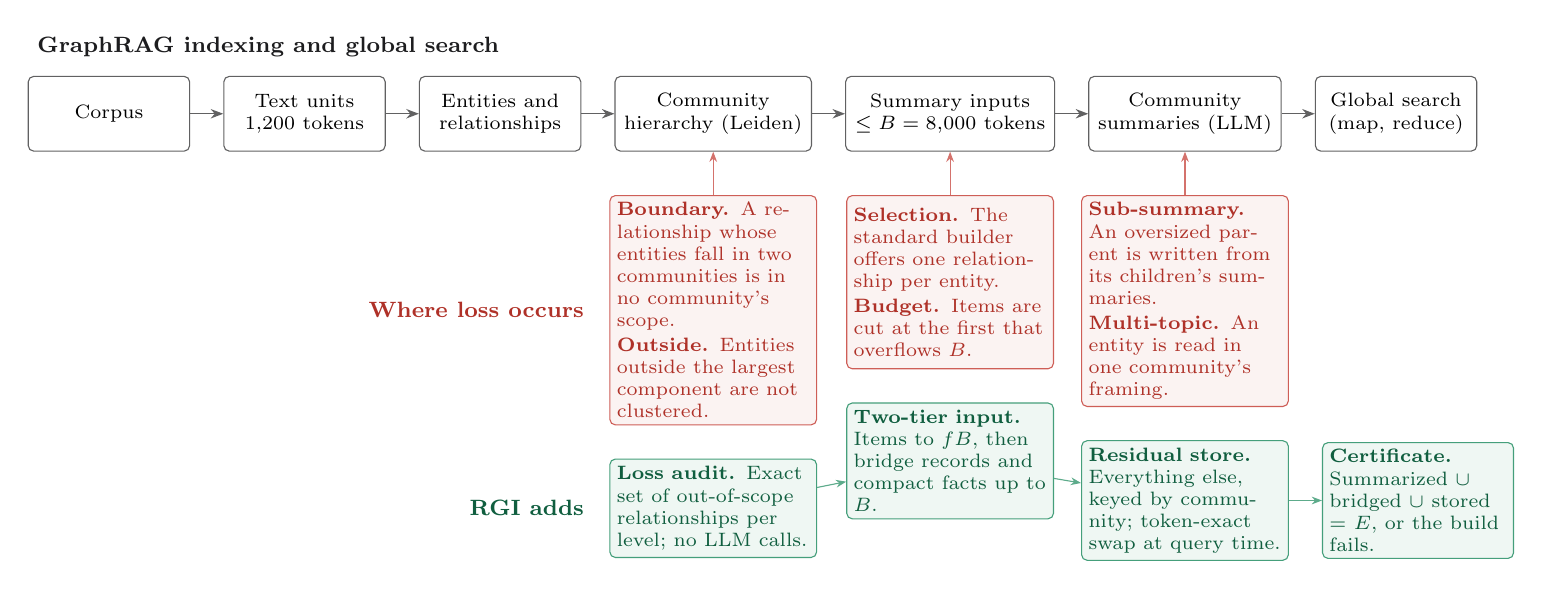
\begin{tikzpicture}[
  font=\scriptsize,
  stage/.style={draw=ink!70, rounded corners=2pt, align=center, minimum width=2.05cm, minimum height=0.95cm, fill=white},
  arr/.style={-{Stealth[length=1.6mm]}, draw=ink!70, line width=0.5pt},
  loss/.style={draw=lost!80, rounded corners=2pt, align=left, fill=lost!6, text=lost!90!black, text width=2.45cm, inner sep=2.5pt, minimum height=2.2cm},
  fix/.style={draw=kept!80, rounded corners=2pt, align=left, fill=kept!7, text=kept!70!black, text width=2.45cm, inner sep=2.5pt, minimum height=1.25cm},
  tag/.style={circle, fill=lost, text=white, inner sep=0.6pt, font=\tiny\bfseries},
]
\node[stage] (s1) {Corpus};
\node[stage, right=0.42cm of s1] (s2) {Text units\\1,200 tokens};
\node[stage, right=0.42cm of s2] (s3) {Entities and\\relationships};
\node[stage, right=0.42cm of s3] (s4) {Community\\hierarchy (Leiden)};
\node[stage, right=0.42cm of s4] (s5) {Summary inputs\\$\le B=8{,}000$ tokens};
\node[stage, right=0.42cm of s5] (s6) {Community\\summaries (LLM)};
\node[stage, right=0.42cm of s6] (s7) {Global search\\(map, reduce)};
\foreach \a/\b in {s1/s2,s2/s3,s3/s4,s4/s5,s5/s6,s6/s7} \draw[arr] (\a) -- (\b);
\node[font=\footnotesize\bfseries, anchor=south west, text=ink] at ($(s1.north west)+(0,0.12)$) {GraphRAG indexing and global search};

\node[loss, below=0.55cm of s4, anchor=north] (l1) {\textbf{Boundary.} A relationship whose entities fall in two communities is in no community's scope.\\[1pt]\textbf{Outside.} Entities outside the largest component are not clustered.};
\node[loss, below=0.55cm of s5, anchor=north] (l2) {\textbf{Selection.} The standard builder offers one relationship per entity.\\[1pt]\textbf{Budget.} Items are cut at the first that overflows $B$.};
\node[loss, below=0.55cm of s6, anchor=north] (l3) {\textbf{Sub-summary.} An oversized parent is written from its children's summaries.\\[1pt]\textbf{Multi-topic.} An entity is read in one community's framing.};
\draw[draw=lost!70, -{Stealth[length=1.3mm]}] (l1.north) -- (s4.south);
\draw[draw=lost!70, -{Stealth[length=1.3mm]}] (l2.north) -- (s5.south);
\draw[draw=lost!70, -{Stealth[length=1.3mm]}] (l3.north) -- (s6.south);

\node[fix, below=0.42cm of l1] (f1) {\textbf{Loss audit.} Exact set of out-of-scope relationships per level; no LLM calls.};
\node[fix, below=0.42cm of l2] (f2) {\textbf{Two-tier input.} Items to $fB$, then bridge records and compact facts up to $B$.};
\node[fix, below=0.42cm of l3] (f3) {\textbf{Residual store.} Everything else, keyed by community; token-exact swap at query time.};
\node[fix, right=0.42cm of f3, text width=2.25cm] (f4) {\textbf{Certificate.} Summarized $\cup$ bridged $\cup$ stored $=E$, or the build fails.};
\draw[draw=kept!70, -{Stealth[length=1.3mm]}] (f1) -- (f2);
\draw[draw=kept!70, -{Stealth[length=1.3mm]}] (f2) -- (f3);
\draw[draw=kept!70, -{Stealth[length=1.3mm]}] (f3) -- (f4);
\node[font=\footnotesize\bfseries, anchor=east, text=kept!70!black] at ($(f1.west)+(-0.2,0)$) {RGI adds};
\node[font=\footnotesize\bfseries, anchor=east, text=lost!90!black] at ($(l1.west)+(-0.2,0)$) {Where loss occurs};
\end{tikzpicture}
\caption{GraphRAG's indexing pipeline, the six places where content leaves the path to an answer, and the four components RGI adds. Summaries, clustering and retrieval are unchanged.}
\label{fig:pipeline}
\end{figure*}

We then propose \emph{Residual Graph Indexing} (RGI). We borrowed the idea from video coding, where a codec stores keyframes and, alongside them, residuals holding whatever the keyframes failed to capture~\cite{wiegand2003h264}. In RGI the community summaries play the part of the keyframes, and GraphRAG writes them exactly as before. What we call the residual is the set of relationships that the summary inputs leave out, and we compute it exactly from the index tables GraphRAG already produces. RGI changes how each input spends its budget, adds bridge records for relationships that cross communities, keeps the remainder in a residual store that query time can use without adding tokens, and checks at build time that every relationship is accounted for.

Our contributions are the following.
\begin{itemize}
\item A loss model for community-summary GraphRAG that separates relationships that are out of scope from relationships whose evidence is absent from every input. It comes with three propositions: absent evidence is unreachable for every summary-reading retrieval policy, boundary loss can only grow toward the leaves of a nested hierarchy, and the standard input builder admits at most $2/\bar d$ of a community's internal relationships, where $\bar d$ is their mean internal degree (Section~\ref{sec:model}).
\item An exact census, run without an LLM through GraphRAG~3.1.1's own code, of all \NNovels{} novels in GraphRAG-Bench Novel~\cite{xiang2026graphragbench} (Sections~\ref{sec:setup} and~\ref{sec:results}).
\item RGI, with four guarantees that we prove and then check on every run: no input exceeds its budget, no relationship that GraphRAG kept in scope is dropped, the number of LLM calls is unchanged, and every relationship is certified as summarized, bridged or stored (Section~\ref{sec:rgi}).
\item A controlled simulation that carries the loss through retrieval to judged answers, and a protocol for the answer-level test whose kill thresholds were committed to version control before any data existed (Sections~\ref{sec:sim} and~\ref{sec:protocol}).
\end{itemize}

We state plainly what this paper does not show. No experiment here measures answer accuracy on an LLM-built index. The census uses GraphRAG's LLM-free fast pipeline with a substitute entity extractor, and the simulation is synthetic. Section~\ref{sec:threats} discusses each limit.

% =====================================================================
\section{Background and Related Work}\label{sec:related}

\subsection{Community-summary GraphRAG}
GraphRAG~\cite{edge2024graphrag,graphrag311} splits documents into text units (1,200 tokens with 100 tokens of overlap by default, counted with the \texttt{o200k\_base} encoding). Its standard pipeline asks an LLM to extract entities and relationships with descriptions. Its fast pipeline extracts noun phrases instead, links phrases that occur in the same text unit, weights the links by pointwise mutual information (PMI) and prunes them. Both pipelines cluster the graph with hierarchical Leiden~\cite{traag2019leiden} as implemented in graspologic~\cite{chung2019graspy}, splitting any community larger than ten entities. Each community then receives a report written by an LLM from a summary input of at most 8,000 tokens (\texttt{max\_input\_length}). Global search at level $\ell$ (the command-line default is $\ell=2$) gives every entity the report of its deepest community at or above level $\ell$ and maps the question over those reports. LazyGraphRAG~\cite{edge2024lazygraphrag} defers summarization to query time.

The original evaluation compared global search at several hierarchy levels with a map-reduce summarization over the source text, which has no partition, and found no significant difference in aggregate answer quality~\cite{edge2024graphrag}. Later evaluations report that graph-based RAG does not uniformly beat chunk retrieval~\cite{han2025ragvsgraphrag,xiang2026graphragbench,zhou2025indepth}, and GraphRAG-Bench reports that global search uses 331,375 tokens per query on its Novel corpus~\cite{xiang2026graphragbench}. We return to the first finding in Section~\ref{sec:discussion}, because an aggregate quality score can hide element-level loss.

\subsection{Other graph-based retrieval}
LightRAG~\cite{guo2024lightrag} retrieves entities and relationships directly at two levels of abstraction and has no community layer. HippoRAG~\cite{gutierrez2024hipporag} runs personalized PageRank over an extracted graph. RAPTOR (recursive abstractive processing for tree-organized retrieval)~\cite{sarthi2024raptor} builds a tree of recursive summaries over chunks. G-Retriever~\cite{he2024gretriever} retrieves subgraphs of textual graphs. ArchRAG~\cite{wang2026archrag} detects communities from links and attributes and indexes them hierarchically. Surveys cover the wider field~\cite{peng2024graphragsurvey}.

\subsection{Work on community boundaries}
Several recent systems target the gaps between communities, mostly at query time (Table~\ref{tab:related}). HiRAG~\cite{huang2025hirag} builds a layered knowledge hierarchy and retrieves the knowledge that connects local entities with global communities. LeanRAG~\cite{zhang2026leanrag} adds explicit relations between aggregated summary nodes, which it calls ``semantic islands'' when unlinked, and retrieves along lowest-common-ancestor paths. Deep GraphRAG~\cite{li2026deepgraphrag} filters across communities, refines within them, and searches entities inside the chosen ones. OMD-GraphRAG (ontology-guided extraction, multi-dimensional clustering and dual-channel fusion)~\cite{wang2026omd} is the closest to our bridge records: an external entity is projected into a community's summary representation when the share of its edges that point into the community exceeds a threshold. Hossain and Sar{\i}y{\"u}ce~\cite{hossain2026core} replace Leiden with $k$-core decomposition, prove that modularity admits exponentially many near-optimal partitions on sparse knowledge graphs, and sample within a token budget.

\begin{table}[!htbp]
\caption{How related systems treat the space between communities}\label{tab:related}
\centering\footnotesize
\begin{tabular}{@{}p{2.05cm}p{0.95cm}p{4.55cm}@{}}
\toprule
System & Acts at & Mechanism \\
\midrule
GraphRAG~\cite{edge2024graphrag} & index & One summary per community; cross-community relationships are out of every scope \\
HiRAG~\cite{huang2025hirag} & index, query & Layered hierarchy; retrieval of connecting knowledge between layers \\
LeanRAG~\cite{zhang2026leanrag} & index, query & Explicit relations among aggregated nodes; path retrieval \\
Deep GraphRAG~\cite{li2026deepgraphrag} & query & Inter-community filtering, then intra-community search \\
OMD-GraphRAG~\cite{wang2026omd} & index & Threshold-based projection of boundary entities into summaries \\
Core hierarchies~\cite{hossain2026core} & index & $k$-core hierarchy replaces Leiden \\
\textbf{RGI (ours)} & index, query & Exact loss audit; budget-neutral bridges and compact facts; residual store; coverage certificate \\
\bottomrule
\end{tabular}
\end{table}

RGI differs in where it starts. It changes neither the clustering nor the retrieval nor the summary prompt. It begins from the exact set of relationships the inputs leave out, spends a fixed share of the existing budget on the most connected of them, and accounts for every relationship. To our knowledge none of the systems above reports an element-level account of what the summaries omit.

\subsection{Compression, granularity and community structure}
RAG systems already trade detail for budget. RECOMP (retrieve, compress, prepend) compresses retrieved documents before generation~\cite{xu2024recomp}, Dense~X retrieval studies the unit of retrieval~\cite{chen2024densex}, and long contexts are used unevenly by the model~\cite{liu2024lost}. That last result is why every comparison in this paper holds the token count fixed: content added on top of a context confounds the content with its length. On the clustering side, modularity has a resolution limit~\cite{fortunato2007resolution} and many near-equivalent optima~\cite{good2010modularity,fortunato2010community}, and some entities connect several modules by nature~\cite{guimera2005cartography}. Partition boundaries are therefore partly arbitrary, which makes it more important to know what they cut.

% =====================================================================
\section{A Model of Index-Time Loss}\label{sec:model}

\subsection{Setting}
The corpus is split into text units $\mathcal U$. Extraction yields a graph $G=(V,E)$, and each relationship $r=(a,b)\in E$ has a support $U(r)\subseteq\mathcal U$, the units it was extracted from. Clustering yields communities $\mathcal C$. Each $c\in\mathcal C$ has a level $\lambda(c)$, with $0$ the coarsest, and the hierarchy is nested: the children of a community partition its entities. Global search at level $\ell$ reads the summaries of
\begin{equation}
S_\ell=\{\Sel(v): v\in V\},\quad \Sel(v)=\arg\max_{c\ni v,\ \lambda(c)\le\ell}\lambda(c),
\end{equation}
so every entity is read through its deepest community at or above level $\ell$; $\Sel(v)$ is undefined for an entity that was never clustered. GraphRAG implements this roll-up by taking, for each entity, the largest community identifier at levels up to $\ell$. We verified on every census graph that this rule returns the deepest community. Each $c$ has a summary input $\In(c)=\beta(c;B)$ built by an input builder $\beta$ under budget $B$, and a summary $s(c)=M(\In(c))$ written by a model $M$. We write $\tok(x)$ for the number of tokens in a string $x$ under the \texttt{o200k\_base} encoding, so $\tok(\In(c))\le B$. Table~\ref{tab:notation} collects every abbreviation and symbol used in the paper.

\begin{table}[!htbp]
\caption{Abbreviations and symbols}\label{tab:notation}
\centering\footnotesize
\begin{tabular}{@{}p{2.15cm}p{5.65cm}@{}}
\toprule
\multicolumn{2}{@{}l}{\emph{Abbreviations}} \\
CI & confidence interval \\
G1 to G4 & the four pre-registered kill criteria (Table~\ref{tab:gates}) \\
LCC & largest connected component \\
LLM & large language model \\
NLI & natural language inference \\
NLTK & Natural Language Toolkit \\
PMI & pointwise mutual information \\
RAG & retrieval-augmented generation \\
RGI & Residual Graph Indexing, the method of this paper \\
\midrule
\multicolumn{2}{@{}l}{\emph{Graph and index}} \\
$G=(V,E)$ & extracted graph with entities $V$ and relationships $E$ \\
$r=(a,b)$ & relationship between entities $a$ and $b$ \\
$\mathcal U$, $U(r)$ & text units; the units that support $r$ \\
$\mathcal C$, $c$, $\lambda(c)$ & communities; one community; its level ($0$ is the coarsest) \\
$\ell$ & query level of global search \\
$\Sel(v)$, $S_\ell$ & community through which $v$ is read at level $\ell$; all such communities \\
$\In(c)$, $\beta$, $B$ & summary input of $c$; input builder; budget in tokens \\
$s(c)$, $M$ & summary of $c$; summarizing model \\
$\tok(x)$ & number of tokens in $x$ under \texttt{o200k\_base} \\
$L_\ell$ & relationships out of scope at level $\ell$ \\
$R^{G}_\ell$, $R^{\mathrm{RGI}}_\ell$ & relationships in scope and represented under GraphRAG and under RGI \\
$\bar d_{\mathrm{in}}(c)$ & mean number of internal relationships per entity of $c$ \\
$\pi$, $C_\pi(q)$ & retrieval policy; its context for query $q$ \\
\midrule
\multicolumn{2}{@{}l}{\emph{RGI parameters and Algorithm~\ref{alg:rgi}}} \\
$f$, $b$, $m$ & full-item cutoff, bridge share, minimum support \\
$E_{\mathrm{in}}$, $E_{\mathrm{bd}}$ & in-scope and boundary relationships of $c$ \\
$P$, $P_{1..k}$, $k_G$ & GraphRAG's items for $c$; their first $k$; the prefix length GraphRAG admits \\
$X$, $\oplus$, $\mathrm{rep}(X)$ & input under construction; append; relationships represented in $X$ \\
$\prec$ & priority order, higher combined degree first \\
\midrule
\multicolumn{2}{@{}l}{\emph{Evaluation}} \\
$Y(q)$ & gold relationships of question $q$ \\
$K$ & summaries read per question (simulation) \\
$\kappa$ & Cohen's agreement coefficient \\
\bottomrule
\end{tabular}
\end{table}

A relationship is \emph{in scope} for $c$ if both entities belong to $c$. It is \emph{represented} in $\In(c)$ if its record appears there (standard pipeline) or one of its supporting text units does (fast pipeline).

\begin{definition}[Status]\label{def:status}
At level $\ell$ every $r=(a,b)\in E$ has exactly one status. It is \emph{outside} if $\Sel(a)$ or $\Sel(b)$ is undefined, and \emph{boundary} if $\Sel(a)\ne\Sel(b)$. Otherwise let $c=\Sel(a)=\Sel(b)$. Then $r$ is \emph{represented} if it is represented in $\In(c)$, \emph{sub-summary} if $\In(c)$ was assembled from the summaries of $c$'s children, \emph{selection} if $\beta$ never offered $r$, and \emph{budget} if $\beta$ offered $r$ and cut it at $B$.
\end{definition}

Out of scope at level $\ell$ means any status other than represented, and $L_\ell\subseteq E$ denotes the set of relationships out of scope at level $\ell$. Scope is a property of the index structure. Evidence is a separate question, because one text unit can support many relationships and an entity description can paraphrase relationships it took part in. We therefore grade every relationship by the strongest way its evidence reaches a selected input: \emph{in scope}; \emph{endpoint}, when a supporting unit sits in the input of a community that holds one of its entities; \emph{elsewhere}, when a supporting unit sits only in inputs about other entities; and \emph{absent}, when no record and no supporting unit appears in any input in $S_\ell$. A sixth kind of loss is entity-level: an entity whose text units span several topics is filed under one community and read in that framing only. We call it \emph{multi-topic} loss. It does not remove the entity from the index, so it falls outside the propositions below.

\subsection{Three propositions}

\begin{proposition}[Absent evidence is unreachable]\label{prop:unreach}
Fix a level $\ell$ and any retrieval policy $\pi$ whose context $C_\pi(q)$ for a query $q$ is a function of $q$ and $\{s(c):c\in S_\ell\}$. If the evidence of $r$ is absent at level $\ell$, then $C_\pi(q)$ does not change when the units in $U(r)$ are edited, for every $q$.
\end{proposition}
\begin{proof}
The corpus can influence a summary $s(c)$ only through its input $\In(c)$. If $r$'s evidence is absent, no unit of $U(r)$ and no record derived from it appears in any $\In(c)$ with $c\in S_\ell$, so editing those units leaves every input, every summary and therefore $C_\pi(q)$ unchanged.
\end{proof}

Proposition~\ref{prop:unreach} is deliberately narrow. It covers absent evidence, not everything out of scope. A relationship that is out of scope but whose supporting text sits in some input can still be mentioned by a summary, and a description of an entity can mention a relationship that has no record of its own. How often that happens is an empirical question about the summarizer. Gate G1, the first of the four pre-registered kill criteria G1 to G4 in Section~\ref{sec:protocol}, is designed to measure it.

\begin{proposition}[Boundary loss grows toward the leaves]\label{prop:mono}
On a nested hierarchy, if $\ell<\ell'$ then every relationship with status boundary at level $\ell$ has status boundary at level $\ell'$.
\end{proposition}
\begin{proof}
Two distinct communities of a nested hierarchy are either disjoint or one contains the other. Suppose $\Sel(a)\ne\Sel(b)$ and $\Sel(a)\supsetneq\Sel(b)$. Then $\Sel(a)$ has children, the child holding $a$ sits at a level no deeper than $\lambda(\Sel(b))\le\ell$, and it is deeper than $\Sel(a)$, which contradicts the choice of $\Sel(a)$. So $\Sel(a)$ and $\Sel(b)$ are disjoint. For every clustered $v$, $\sigma_{\ell'}(v)\subseteq\Sel(v)$, hence $\sigma_{\ell'}(a)$ and $\sigma_{\ell'}(b)$ are disjoint as well.
\end{proof}

Coarser levels pay for fewer boundaries with larger inputs. With a fixed $B$, the share of inputs that overflow, and that must be truncated or assembled from child summaries, can only rise as communities merge. Proposition~\ref{prop:mono} and this budget effect pull in opposite directions, which is the trade-off the census measures.

\begin{proposition}[Selection bound]\label{prop:select}
In GraphRAG~3.1.1's standard input builder, at most $|c|$ of the relationships in scope for a community $c$ can be represented in $\In(c)$, whatever $B$ is. The represented share of $c$'s internal relationships is therefore at most $2/\bar d_{\mathrm{in}}(c)$, where $\bar d_{\mathrm{in}}(c)$ is the mean number of internal relationships per entity of $c$.
\end{proposition}
\begin{proof}
Inside \texttt{\_prepare\_reports\_at\_level}, the relationships of the level are grouped twice, once by source entity and once by target entity. Only the first relationship in each group survives, and the two resulting tables are merged with \texttt{combine\_first}, so an entity contributes one relationship record at most and $\In(c)$ can offer no more than $|c|$ records. Because $c$ has $|c|\,\bar d_{\mathrm{in}}(c)/2$ internal relationships, the represented share cannot exceed $2/\bar d_{\mathrm{in}}(c)$.
\end{proof}

In practice the real share is lower still. The one record an entity contributes may point to an entity in another community, and two entities can end up contributing the same record. With an internal degree close to 2, as in a sparse graph, the bound hardly matters, whereas on a dense graph the cap removes most of the relationships.

% =====================================================================

% =====================================================================
\section{Residual Graph Indexing}\label{sec:rgi}

\subsection{Requirements}
RGI was designed under four requirements. The first two keep the comparison fair. GraphRAG's clustering, summary prompt and global search stay exactly as they are, and no input or query context gets a larger token budget, because extra tokens alone change how a model behaves~\cite{liu2024lost}. With both held fixed, any difference in results has to come from what the inputs contain. The other two concern cost and accounting: indexing may not need any extra LLM call, and the method has to be able to report, for each relationship, where it ended up. Fig.~\ref{fig:pipeline} shows the four components we built to meet these requirements.

\subsection{Loss audit}
For each level $\ell$, the audit gives every relationship one of the statuses of Definition~\ref{def:status}. Finding the boundary and outside relationships needs only a set difference on tables GraphRAG already writes, namely all relationship identifiers minus the ones listed inside the selected communities. The budget and selection statuses are obtained by replaying the input builder with GraphRAG's own sort key, budget and tokenizer, and because the builder is deterministic the replay is exact. No model is called during the audit, and apart from tokenization its cost per level grows linearly with $|E|$.

\subsection{Two-tier summary input}
GraphRAG adds items to an input in priority order until one of them would overflow $B$. It stops there, and every remaining item is dropped together. RGI uses the same items in the same order and differs only in how it spends the last part of the budget (Algorithm~\ref{alg:rgi}, Fig.~\ref{fig:layout}). An input that already fits within $B$ is kept whole, and whatever slack is left goes to bridge records. For an input that overflows, RGI keeps full items only up to a cutoff $fB$ and fills the space after it with one-line \emph{compact facts} of the form \texttt{source,target,support}, in GraphRAG's own priority order (highest combined degree first).

\begin{figure}[!htbp]
\centering
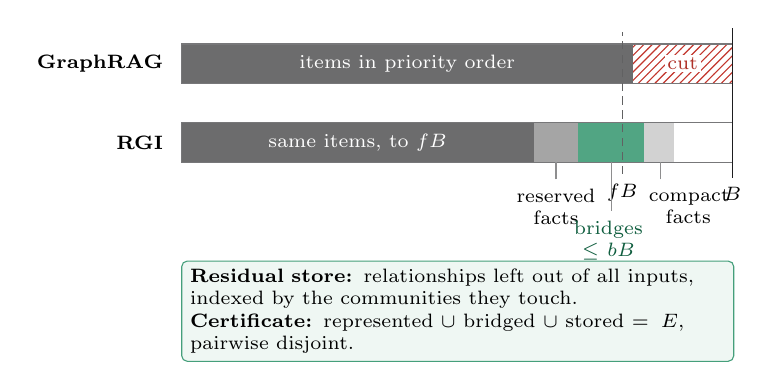
\begin{tikzpicture}[font=\scriptsize, x=0.70cm]
% GraphRAG input
\node[anchor=east, font=\scriptsize\bfseries] at (-0.15,1.45) {GraphRAG};
\fill[ink!65] (0,1.2) rectangle (8.2,1.7);
\fill[pattern=north east lines, pattern color=lost] (8.2,1.2) rectangle (10,1.7);
\draw[ink!60] (0,1.2) rectangle (10,1.7);
\node[text=white] at (4.1,1.45) {items in priority order};
\node[text=lost!90!black, fill=white, inner sep=1pt] at (9.1,1.45) {cut};
% RGI input
\node[anchor=east, font=\scriptsize\bfseries] at (-0.15,0.45) {RGI};
\fill[ink!65] (0,0.2) rectangle (6.4,0.7);
\fill[ink!40] (6.4,0.2) rectangle (7.2,0.7);
\fill[kept!75] (7.2,0.2) rectangle (8.4,0.7);
\fill[ink!20] (8.4,0.2) rectangle (8.95,0.7);
\draw[ink!60] (0,0.2) rectangle (10,0.7);
\node[text=white] at (3.2,0.45) {same items, to $fB$};
\draw[densely dashed, ink!70] (8.0,0.05) -- (8.0,1.85);
\draw[ink] (10,0.0) -- (10,1.9);
\node[anchor=north] at (10,0.0) {$B$};
\node[anchor=north] at (8.0,0.05) {$fB$};
\node[anchor=north, text width=1.1cm, align=center] at (6.8,-0.02) {reserved facts};
\node[anchor=north, text width=1.0cm, align=center, text=kept!70!black] at (7.75,-0.42) {bridges $\le bB$};
\node[anchor=north, text width=1.0cm, align=center] at (9.2,-0.02) {compact facts};
\draw[ink!50] (7.8,-0.42) -- (7.8,0.2);
\draw[ink!50] (8.7,-0.02) -- (8.7,0.2);
\draw[ink!50] (6.8,-0.02) -- (6.8,0.2);
% residual
\node[draw=kept!80, fill=kept!7, rounded corners=2pt, align=left, text width=6.8cm, anchor=north west, inner sep=3pt] at (0,-1.05)
  {\textbf{Residual store:} relationships left out of all inputs, indexed by the communities they touch.\\
   \textbf{Certificate:} represented $\cup$ bridged $\cup$ stored $=E$, pairwise disjoint.};
\end{tikzpicture}
\caption{Layout of one summary input. GraphRAG adds items until the first one that overflows $B$ and drops everything from there on. RGI stops full items at $fB$. In the space that remains it first writes compact facts for whatever the shorter prefix lost, then bridge records, then further compact facts, and the total stays within $B$.}
\label{fig:layout}
\end{figure}

A compact fact costs about ten tokens and a text unit about 1,200. What facts give up is detail, since a fact records only that two entities are related and says nothing about the relation itself. The first facts RGI writes are reserved for relationships that GraphRAG's own input represented and that the shortened prefix has lost. Should these reserved facts not fit, RGI keeps GraphRAG's own input for that community and uses only the leftover slack; the monotonicity guarantee below depends on this rule. For communities whose input is assembled from child summaries, the child summaries are capped at $fB$ instead of $B$, and the tail holds compact facts about the community's own relationships.

Algorithm~\ref{alg:rgi} uses the following notation. $P$ is GraphRAG's list of items for $c$ in its own order, $P_{1..k}$ its first $k$ items, and $k_G$ the length of the prefix GraphRAG admits under $B$. $X$ is the input under construction and $\oplus$ appends to it. $\mathrm{rep}(X)$ is the set of relationships represented in $X$; $\mathrm{fact}(r)$, $\mathrm{facts}(Q)$ and $\mathrm{bridge}(r)$ render one-line records for a relationship $r$ or a set $Q$; $\textit{pend}$ holds the in-scope relationships still waiting for a compact fact; and $r\prec r'$ means that $r$ has the higher combined degree.

\begin{algorithm}[!htbp]
\caption{RGI summary input for community $c$ at level $\ell$}\label{alg:rgi}
\footnotesize
\begin{algorithmic}[1]
\Require items $P$ in GraphRAG order; in-scope set $E_{\mathrm{in}}$; boundary set $E_{\mathrm{bd}}$; budget $B$; cutoff $f$; bridge share $b$; support $m$; priority $\prec$
\State $k_G\gets$ GraphRAG's admitted prefix length under $B$
\If{$\tok(P)\le B$} $X\gets P$; $\textit{pend}\gets\emptyset$
\Else
  \State $k\gets$ longest prefix with $\tok(P_{1..k})\le fB$ \Comment{$k\le k_G$}
  \State $Q\gets\mathrm{rep}(P_{1..k_G})\setminus\mathrm{rep}(P_{1..k})$ sorted by $\prec$ \Comment{reserved}
  \If{$\tok(P_{1..k}\oplus\mathrm{facts}(Q))>B$} $k\gets k_G$; $Q\gets\emptyset$ \Comment{fallback}
  \EndIf
  \State $X\gets P_{1..k}\oplus\mathrm{facts}(Q)$; $\textit{pend}\gets E_{\mathrm{in}}\setminus\mathrm{rep}(P_{1..k_G})$
\EndIf
\For{$r\in E_{\mathrm{bd}}$ with $|U(r)|\ge m$, in $\prec$ order}
  \If{bridge tokens would exceed $\min(bB,\,B-\tok(X))$} \textbf{break} \EndIf
  \State append $\mathrm{bridge}(r)$ to $X$
\EndFor
\For{$r\in\textit{pend}$ in $\prec$ order}
  \If{$\tok(X\oplus\mathrm{fact}(r))>B$} \textbf{break} \EndIf
  \State append $\mathrm{fact}(r)$ to $X$
\EndFor
\While{$\tok(\mathrm{render}(X))>B$} drop the last fact of $X$ \EndWhile
\State residual$(c)\gets(E_{\mathrm{in}}\cup E_{\mathrm{bd}})\setminus\mathrm{rep}(X)$
\State \Return $X$
\end{algorithmic}
\end{algorithm}

\subsection{Bridge records}
Each community spends at most a share $b$ of $B$ on \emph{bridge records}: boundary relationships with at least $m$ supporting text units, ranked by combined degree and written as compact facts into the inputs of both endpoint communities. A relationship counts as bridged if it lands in at least one of the two. Bridges use the description GraphRAG already extracted when one exists, so no summary is rewritten and no model is called.

\subsection{Residual store and query-time substitution}
Every relationship that is neither represented nor bridged goes to a residual store keyed by the communities it touches (or by a global key, for outside relationships). After global search selects its reports, RGI can add the stored facts of those communities that best match the question. Added facts \emph{replace} the lowest-ranked context so that the token count of the context stays exactly the same. Our implementation of this swap holds token counts equal under \texttt{o200k\_base} on 50 random contexts, 10 contexts with mixed scripts and punctuation, and five insertion sizes from 5\% to 95\% of the context.

\subsection{Coverage certificate}
At build time RGI checks, for every level, that the represented, bridged and stored sets are disjoint and that their union is $E$. A failure stops the build. GraphRAG today discards content without a record; the certificate makes the discard visible and bounded, and it would also flag loss from a mechanism nobody anticipated, such as the selection behavior of Proposition~\ref{prop:select}.

\subsection{Guarantees}
Let $R^G_\ell$ and $R^{\mathrm{RGI}}_\ell$ be the relationships in scope and represented under GraphRAG and under RGI at level $\ell$.

\begin{proposition}[Guarantees]\label{prop:guarantees}
For every community and level: (i) $\tok(\In_{\mathrm{RGI}}(c))\le B$; (ii) $R^G_\ell\subseteq R^{\mathrm{RGI}}_\ell$; (iii) RGI makes exactly one summarization call per community, as GraphRAG does; (iv) the represented, bridged and stored sets partition $E$.
\end{proposition}
\begin{proof}
(i) The final loop of Algorithm~\ref{alg:rgi} enforces the bound on the rendered string with the production tokenizer. (ii) If the input fits, $X$ contains all of $P$. Otherwise either the reserved facts $Q$ restore every relationship that $P_{1..k_G}$ represented and $P_{1..k}$ did not, or the fallback restores $P_{1..k_G}$ itself; bridges and later facts only add. Reserved facts precede all other appended lines, so the final loop reaches them only if $P_{1..k}\oplus\mathrm{facts}(Q)$ alone overflows. The fallback test excludes that case up to tokenizer merges at line boundaries, and we check the outcome on every run. (iii) RGI changes inputs, not the number of summaries. (iv) Each relationship is placed in the residual store exactly when it is neither represented nor bridged.
\end{proof}

The guarantee in (ii) is about relationships in scope. When an input overflows, RGI swaps GraphRAG's last full items for compact facts, so the text of those items is no longer in the input, and a relationship that was only incidentally exposed through that text can lose its exposure. The census counts these cases.

% =====================================================================
\section{Experimental Setup}\label{sec:setup}

\subsection{Corpus}
GraphRAG-Bench~\cite{xiang2026graphragbench} provides two corpora. We use Novel: \NNovels{} pre-twentieth-century novels from Project Gutenberg, chosen by the benchmark's authors to limit overlap with pretraining data, totalling \NChars{} characters and \NTokens{} tokens. It comes with \NQuestions{} questions in four types (fact retrieval, complex reasoning, contextual summarization, creative generation), each with gold evidence given as sentences and as $(\textit{head},\textit{relation},\textit{tail})$ triples. The data are released under the MIT license.

\subsection{Index construction}
We index each novel separately with GraphRAG~3.1.1's fast pipeline at its shipped defaults (Table~\ref{tab:corpus}). Every stage except one calls GraphRAG's own functions: the token chunker, the co-occurrence edge builder with PMI weights, \texttt{prune\_graph} (minimum frequency 2, minimum edge weight at the 40th percentile, removal of the single most connected entity), hierarchical Leiden with maximum community size 10 and the default seed, and the text-unit input builder with its degree ordering and first-overflow cut. The exception is noun-phrase extraction. GraphRAG's default extractor needs tagger data from the Natural Language Toolkit (NLTK) that we could not download on our network, so we substitute a deterministic proper-noun extractor that keeps the default extractor's output format, stop words and token rules (Section~\ref{sec:threats}). No LLM is called anywhere; a full run over the corpus, including every configuration reported here, takes \RuntimeS{} seconds on an Apple M2 laptop.

\begin{table}[!htbp]
\caption{Census corpus and index (GraphRAG 3.1.1 fast pipeline)}\label{tab:corpus}
\centering\footnotesize
\begin{tabular}{@{}lr@{}}
\toprule
Novels / questions & \NNovels{} / \NQuestions{} \\
Text units (1,200 tokens, 100 overlap) & \NUnits{} \\
Extracted entities / relationships & \NRawEntities{} / \NRawRels{} \\
After pruning: entities / relationships & \NEntities{} / \NRels{} \\
Mean degree (pooled; median over novels) & \MeanDegree{} (\MedianDegree{}) \\
Communities, all levels & \NCommunities{} \\
Deepest level reached & \MaxLevelMax{} \\
Summary input budget $B$ & 8,000 tokens (\texttt{o200k\_base}) \\
Largest novel's share of relationships & \BigNovelShare\% \\
LLM calls & 0 \\
\bottomrule
\end{tabular}
\end{table}

To make sure we measure GraphRAG's behavior and not our reading of it, we compared our admission logic with GraphRAG's own \texttt{sort\_context} on \EquivChecks{} overflowing communities; the admitted text was identical in every case. The standard pipeline's input builder is run unchanged in Section~\ref{sec:select}.

\subsection{Measurements}
For each novel, level $\ell\in\{0,1,2,3\}$ and budget $B\in\{4\mathrm{k},8\mathrm{k},16\mathrm{k},32\mathrm{k}\}$ we record each relationship's status (Definition~\ref{def:status}) and evidence grade under GraphRAG and under RGI. A census counts every relationship, so we report counts and proportions without $p$-values. Because one novel holds \BigNovelShare\% of all relationships, we report both the pooled share and the mean of per-novel shares, the latter with a 95\% bootstrap confidence interval (CI) over novels (10,000 resamples)~\cite{efron1979bootstrap}.

\subsection{Gold evidence}
We link gold triples to the graph with the parameters frozen before any data were collected: both head and tail must reach a \texttt{token\_set\_ratio} of at least 85 against an entity title of the question's own novel, and a triple whose endpoints link identifies the relationships between them. For a question $q$ we write $Y(q)\subseteq E$ for the relationships its triples resolve to, and $q$ enters the gold analysis when $Y(q)$ is not empty. The quantity of interest is the share of such questions with $Y(q)\cap L_\ell\neq\emptyset$, that is, with at least one gold relationship out of scope. Our pre-registration also froze a rule: if more than 15\% of triples fail to link, the gold-intersection gate (G2 in Section~\ref{sec:protocol}) is reported as inconclusive. We apply that rule here.

\subsection{RGI configuration}
The defaults are $f=0.8$, $b=0.12$ and $m=2$. The first two were fixed in our design document before any real-data run; $m$ was fixed before the full census. Section~\ref{sec:ablate} reports every value we tried.

% =====================================================================
\section{Results}\label{sec:results}

\subsection{How much each level loses}\label{sec:census}
The census results are in Table~\ref{tab:census} and Fig.~\ref{fig:census}. At the default level~2, GraphRAG's inputs keep only \CovCG\% of relationships in scope, and boundaries account for \BndCG\%. Almost nothing is lost to the budget at this level, because nearly every community there is a leaf with ten entities or fewer and its input fits. The root level looks very different. Only \CovAG\% stays in scope there, \BndAG\% crosses a boundary, and \IndAG\% of relationships belong to communities whose inputs are built from child summaries. From level~0 to level~3, boundary loss rises monotonically, which is what Proposition~\ref{prop:mono} predicts.

\begin{table}[!htbp]
\caption{Share of relationships (\%) by status at $B=8{,}000$, pooled over novels. Bnd.\ = boundary, Sub.\ = sub-summary only, Bud.\ = budget. The last column is the mean over novels of RGI's in-scope share minus GraphRAG's, with a 95\% bootstrap interval. Level~2 is the default.}\label{tab:census}
\centering\footnotesize
\input{generated/tab_census}
\end{table}

\begin{figure}[!htbp]
\centering
\includegraphics[width=\columnwidth]{figures/fig_census.pdf}
\caption{Where every relationship ends up at each query level, pooled over \NNovels{} novels. Black, grey and green segments are in scope and red segments are out of scope. LCC = largest connected component. Since RGI leaves the clustering alone and only changes how inputs use their budget, the boundary segment shrinks only by the relationships that bridge records carry.}
\label{fig:census}
\end{figure}

Scope is not the same as evidence (Table~\ref{tab:exposure}). In the fast pipeline an input is made of text units, and one unit names many entities. At level~2, \NearCG\% of relationships have a supporting unit in the input of a community that holds one of their entities, and only \AbsCG\% have no evidence in any input. At level~0 the inputs of oversized communities hold no raw text at all, and \AbsAG\% of relationships have no evidence anywhere. Proposition~\ref{prop:unreach} applies to exactly these relationships. The fast pipeline therefore loses evidence mostly at coarse levels, through second-hand summarization, and loses scope mostly at fine levels, through boundaries.

\begin{table}[!htbp]
\caption{Strongest form in which evidence reaches a selected input (\%), $B=8{,}000$; the tiers are those of Section~\ref{sec:model}}\label{tab:exposure}
\centering\footnotesize
\input{generated/tab_exposure}
\end{table}

\subsection{Selection in the standard pipeline}\label{sec:select}
The fast pipeline's text-unit builder does not filter relationships, but the graph builder of the standard pipeline does. We ran GraphRAG's own \texttt{explode\_communities}, \texttt{\_prep\_nodes}, \texttt{\_prep\_edges} and \texttt{build\_local\_context} on the census graphs. Descriptions were left as GraphRAG's own placeholder, which is safe because the selection step never reads them. As Table~\ref{tab:selection} shows, only \SelMin\% to \SelMax\% of within-community relationships make it into their community's input at any level, before any budget is applied. Over all levels the builder also puts \SelCrossTotal{} cross-community relationships into inputs, which happens when the single record an entity contributes points to an entity outside its community.

\begin{table}[!htbp]
\caption{Within-community relationships reaching the standard pipeline's summary input (GraphRAG 3.1.1 \texttt{build\_local\_context}). Comm.\ = communities; Intra rels = within-community relationships; Cross rels in = cross-community relationships placed in inputs}\label{tab:selection}
\centering\footnotesize
\input{generated/tab_selection}
\end{table}

With a mean degree of \MeanDegree, our graphs are dense, and Proposition~\ref{prop:select} cuts deeply. Graphs extracted by an LLM are usually much sparser, so the same code would remove fewer relationships from them, and a practitioner can estimate how many from the mean internal degree alone. The issue report~\cite{grenat2026issue} traces the behavior back to version 0.9.0. A fix has been proposed and linked to that issue, although it had not been merged when we wrote this paper.

\subsection{Recovery at an unchanged budget}\label{sec:recover}
Table~\ref{tab:census} shows a higher in-scope share under RGI at every level. At the root it goes from \CovAG\% to \CovAR\%, and at level~2 from \CovCG\% to \CovCR\%; to get there at level~2, RGI writes \BridgeC{} bridge records and \CompactC{} compact facts over the whole corpus. With each novel weighted equally, the level~2 gain is \MacroDiffC{} points (95\% CI [\MacroDiffCLo, \MacroDiffCHi]). We also checked the guarantees on all \CensusConfigs{} combinations of novel, level, budget and configuration. None of the relationships GraphRAG kept in scope was pushed out of scope by RGI (\Regressions{} regressions), and Algorithm~\ref{alg:rgi} never had to fall back (\Fallbacks{} times). At $B=8{,}000$ no input went over \MaxTokensRGI{} tokens, and the certificate held in every run.

Absent evidence, the case covered by Proposition~\ref{prop:unreach}, also drops under RGI at the coarse levels; at level~0 its share falls from \AbsAG\% to \AbsAR\%. Level~2 had little absent evidence to begin with, so the change there is small (\AbsCG\% to \AbsCR\%). The two-tier layout does have a cost. Of the \PassCG{} text units GraphRAG admits at level~2, RGI keeps \PassCR{} and uses the space of the others for compact facts. Some relationships were visible only incidentally, through text in the units that were dropped, and they lose that visibility. Summed over the four levels at $B=8{,}000$ this happened \ExpoRegrEight{} times, and at no level did it affect more than \ExpoRegrMaxShare\% of relationships. None of these relationships went out of scope.

The budget sweep in Fig.~\ref{fig:budget} shows that, at fine levels, raising the budget does less than RGI does. With only 4,000 tokens, RGI keeps \BudgetCFourR\% of level~2 relationships in scope, which is more than GraphRAG manages with 32,000 (\BudgetCThirtyTwoG\%). The root behaves differently because its inputs overflow, and there a larger budget does help: over the same range GraphRAG's share climbs from \BudgetAFourG\% to \BudgetAThirtyTwoG\% and RGI's from \BudgetAFourR\% to \BudgetAThirtyTwoR\%.

\begin{figure}[!htbp]
\centering
\includegraphics[width=\columnwidth]{figures/fig_budget.pdf}
\caption{In-scope share as the summary input budget grows from 4k to 32k tokens. At level~2, RGI with 4k tokens already keeps more relationships in scope than GraphRAG with 32k.}
\label{fig:budget}
\end{figure}

\subsection{Do questions need the lost content?}\label{sec:gold}
Of the \NTriples{} gold triples, \TripleParsed\% could be parsed and \TripleLinked\% linked at both endpoints, while \TripleRel\% resolved to a relationship in the graph. That puts the unlink rate at \UnlinkRate\%, well over the 15\% limit we pre-registered, and by our own rule this section therefore cannot count as gate~G2. What it can do is describe the \NGoldQ{} questions (\GoldQShare\% of the benchmark) whose gold evidence does resolve. These questions are skewed toward prominent entities, which the extractor picks up more reliably and which RGI's priority order also favors.

With that caveat, Table~\ref{tab:gold} and Fig.~\ref{fig:gold} show that at level~2, \GoldLostCG\% of these questions have at least one gold relationship out of scope under GraphRAG and \GoldLostCR\% under RGI. The pattern holds for all four question types. Evidence tells a different story by level. At level~2, \GoldAnyCG\% of gold relationships have a supporting unit in some input under GraphRAG, so their loss is a loss of scope. At the root only \GoldAnyAG\% do, against \GoldAnyAR\% under RGI, and the share of these questions with at least one gold relationship whose evidence is absent everywhere falls from \GoldAbsQAG\% to \GoldAbsQAR\%.

\begin{table}[!htbp]
\caption{Questions with at least one gold relationship out of scope (\%), among the \NGoldQ{} questions whose gold evidence resolves}\label{tab:gold}
\centering\footnotesize
\input{generated/tab_gold}
\end{table}

\begin{figure}[!htbp]
\centering
\includegraphics[width=\columnwidth]{figures/fig_gold.pdf}
\caption{Share of questions with a gold relationship out of scope, by query level, among questions whose gold evidence links to the graph.}
\label{fig:gold}
\end{figure}

\subsection{Sensitivity and ablations}\label{sec:ablate}
Graph density follows from the co-occurrence window. Shrinking text units from 1,200 to 600 and 300 tokens lowers the mean degree from \ChunkDefaultDeg{} to \ChunkSixDeg{} and \ChunkThreeDeg{} (Table~\ref{tab:chunk}). GraphRAG's in-scope share at level~2 rises from \ChunkDefaultG\% to \ChunkSixG\% and \ChunkThreeG\%, and RGI's from \ChunkDefaultR\% to \ChunkSixR\% and \ChunkThreeR\%, with no regressions at any size. The size of the loss depends on the graph; its existence and RGI's gain do not.

\begin{table}[!htbp]
\caption{Sensitivity to text-unit size (in-scope share, \%, $B=8{,}000$)}\label{tab:chunk}
\centering\footnotesize
\input{generated/tab_chunk}
\end{table}

Table~\ref{tab:ablation} varies one parameter at a time. At level~2, where most inputs fit, bridge records carry most of the gain: without them RGI reaches only \AblNoBridgeA\% through compact facts in the few overflowing inputs. The minimum support $m$ matters more than the share $b$: moving $b$ from 0.06 to 0.24 changes the in-scope share from \AblBSixA\% to \AblBTwentyFourA\%, while moving $m$ from 3 to 1 changes it from \AblMThreeA\% to \AblMOneA\%. At the root, bridges and compact facts compete for the same tail of the budget. Removing bridges raises the in-scope share there (\AblNoBridgeC\% against \AblMainC\%), a lower cutoff $f=0.6$ raises it further (\AblFSixC\%) by giving compact facts more room, and without the compact tier ($f=1.0$) RGI keeps only \AblFOneC\%. The best allocation therefore depends on the level, a point we return to in Section~\ref{sec:discussion}.

\begin{table}[!htbp]
\caption{Ablations at $B=8{,}000$ (\% of relationships). $b$ = bridge share, $f$ = full-item cutoff, $m$ = minimum support; defaults $b=0.12$, $f=0.8$, $m=2$}\label{tab:ablation}
\centering\footnotesize
\input{generated/tab_ablation}
\end{table}

\subsection{From loss to answers: a controlled simulation}\label{sec:sim}
The census stops at the summary input. To see how loss could propagate to answers we built GraphRAG X-Ray, an interactive simulation that we also use for demonstration. It models a synthetic index shaped like George Eliot's \emph{Middlemarch}: \SimCoreEntities{} entities and \SimCoreRels{} relationships taken from the novel's plot, plus a generated long tail, giving \SimEntities{} entities and \SimRels{} relationships in 22 leaf communities nested into 8, 3 and 1 above them. Token costs, weights and the long tail are generated. Inputs follow GraphRAG's first-overflow rule with its priority order. Retrieval reads the top $K=3$ summaries, ranked by entity overlap with the question, a size prior and noise shared by both methods. A stochastic judge marks an answer correct with probability 0.8, 0.45 or 0.15 when all, at least half, or less than half of the evidence was retrieved. There are \SimQuestions{} questions: \SimFeatured{} written by hand and the rest sampled as paths of two to four relationships. The simulated RGI applies the two-tier layout to every input, a simpler variant of Algorithm~\ref{alg:rgi}.

Table~\ref{tab:sim} and Fig.~\ref{fig:sim} give the outcome. RGI retrieves more evidence at every level. At the leaf level the paired difference lies between \SimCIALo{} and \SimCIAHi{} points (95\% bootstrap CI over questions), and at no level does any question or relationship regress (\SimRegr{} cases). For the original index, reading more summaries hardly helps. Moving from $K=2$ to $K=6$ changes leaf-level evidence retrieval only from \SimKTwoO\% to \SimKSixO\%, since the lost relationships are in none of the summaries. As on the real data, the choice of which relationships to bridge matters more than the budget that bridges receive: lowering the bridge threshold from weight 5 to 3 raises retrieval from \SimBMFive\% to \SimBMThree\%, whereas raising the bridge share from 6\% to 24\% leaves it where it was (\SimBSSix\% and \SimBSTwentyFour\%). At the root a larger budget helps both methods, and GraphRAG keeps \SimBudFourO\% with 4,000 tokens and \SimBudSixteenO\% with 16,000. That gain costs tokens on every query, while the residual store adds none. We wrote the simulator ourselves, so these figures illustrate the mechanism only under our own assumptions.

\begin{table}[!htbp]
\caption{Controlled simulation (synthetic data, \SimQuestions{} questions, \%). Orig.\ = original GraphRAG; numbers in parentheses are communities per level}\label{tab:sim}
\centering\footnotesize
\input{generated/tab_sim}
\end{table}

\begin{figure}[!htbp]
\centering
\includegraphics[width=\columnwidth]{figures/fig_sim.pdf}
\caption{Share of evidence retrieved at each level in the simulation. The data are synthetic, and the figure illustrates the mechanism only.}
\label{fig:sim}
\end{figure}

% =====================================================================
\section{Discussion}\label{sec:discussion}

The census separates two kinds of loss that are easy to mix up. At fine levels, boundaries take relationships out of scope, yet in the fast pipeline the text behind them usually still reaches a summarizer writing about one of the two entities, and it is then up to the model whether the report mentions the relationship. At coarse levels the problem is more serious. Summaries written from other summaries drop the evidence itself, and Proposition~\ref{prop:unreach} then applies in full. A study that looks at only one of these losses will either overstate or understate the problem.

RGI works mainly as bookkeeping on top of GraphRAG. Inside the inputs where they matter it writes boundary relationships out explicitly, it brings back relationships that the budget would have dropped, and everything else goes into the residual store. Because the clustering is unchanged, multi-topic loss stays as it was. RGI also has no way of making a summarizer use the material it receives, and its compact facts hold less information than the text they replace. Where the graph has descriptions, a bridge record can include the extracted description, whereas in the fast pipeline it holds only the entity pair and its support.

How the budget should be split depends on the level. At fine levels the slack in an input costs nothing, and bridge records are the only thing RGI can add there. At the root, bridges and compact facts compete for the same space, and in our ablation compact facts gave more. An allocation that adapts to the level, or a learned salience score, would be a natural next step.

Our results also have to be squared with those of Edge et al., who found no significant difference between global search and a summarization baseline that uses no partition~\cite{edge2024graphrag}. That baseline cannot have boundary loss, so their finding suggests that partition loss leaves aggregate answer quality on broad sensemaking questions unchanged. We make a narrower claim, measured element by element. We expect an effect on fact retrieval and on multi-hop questions whose evidence spans communities, and the protocol in Section~\ref{sec:protocol} tests this separately for each question type. LightRAG~\cite{guo2024lightrag}, which has no community layer at all, is competitive on GraphRAG-Bench~\cite{xiang2026graphragbench}. We still think community summaries are worth keeping, because they let a reader navigate a corpus in a way that direct entity retrieval does not, and RGI is an attempt to keep them while accounting for what they cost.

% =====================================================================
\section{Threats to Validity}\label{sec:threats}

Several threats come from the way our graphs were built. GraphRAG's default extractor finds noun phrases, and we replaced it with a proper-noun extractor of our own. It produces the same output format and follows the same stop-word and token rules, but it leaves out multi-word common noun phrases. All later stages run GraphRAG's own code and the selection analysis does not depend on the extractor at all, yet the absolute shares would be different under the default one. Our graphs are also dense, with a mean degree of \MeanDegree, because entities are linked whenever they co-occur in a 1,200-token unit, and density makes both boundary and selection loss larger. The chunk-size sensitivity run puts a bound on this effect without eliminating it. The data are uneven as well: one novel holds \BigNovelShare\% of all relationships, which is why every pooled figure is reported next to per-novel means with intervals.

Other threats concern what we measure. The census uses the fast pipeline, where inputs are text units, whereas in the standard pipeline they are entity and relationship descriptions written by an LLM. We can measure the selection step of the standard builder exactly, but its budget loss depends on how long those descriptions are, and only an LLM run produces them. Measuring scope also leaves two gaps. A relationship that is in an input may still be left out of the summary, and one that is out of scope may still be mentioned in it. Gate G1 measures the second gap, while the first requires the LLM run.

More than half of the gold triples do not link, so the gold analysis covers a biased subset of questions and cannot be read as a test of gate G2. The simulation is synthetic throughout, and that includes its judge. Finally, all of our results describe GraphRAG~3.1.1. If a fix for the selection behavior is merged, the findings of Section~\ref{sec:select} would change, although the audit and the certificate would still apply.

% =====================================================================
\section{Pre-registered Protocol for the Answer-Level Test}\label{sec:protocol}

Everything measured so far happens at index time, and it matters in practice only if it changes the answers. We committed the thresholds in Table~\ref{tab:gates} to version control on 15 August 2026 (commit \texttt{d223de8}), before any corpus was downloaded or any index built, following the logic of preregistration~\cite{nosek2018prereg}; the linking parameters and tokenizer followed in commit \texttt{21e43d8}. Each gate is a kill criterion: if it fires, the claim is dropped and the result is reported as a null.

\begin{table}[!htbp]
\caption{Kill criteria committed before any data existed}\label{tab:gates}
\centering\footnotesize
\begin{tabular}{@{}lp{4.3cm}l@{}}
\toprule
Gate & Question & Stop if \\
\midrule
G1 & Do summaries already paraphrase out-of-scope relationships? Measured by natural language inference (NLI) on 300 stratified edges, once two annotators agree at Cohen's $\kappa\ge0.7$~\cite{cohen1960kappa} & $>70\%$ \\
G2 & Do questions need the lost content? $\Pr[Y(q)\cap L_\ell\ne\emptyset]$ & $<10\%$ \\
G3 & Are failures caused by the index rather than by retrieval or generation? & $<15\%$ \\
G4 & Does restoring the lost content change answers? Oracle minus placebo accuracy, 95\% CI & includes 0 \\
\bottomrule
\end{tabular}
\end{table}

The causal test (G4) compares two injections at an identical token count: the actual lost gold evidence (oracle) and randomly chosen lost relationships of the same size (placebo). Holding the count fixed separates content from length, which a before-and-after comparison cannot do. Accuracy differences are paired by question and reported with bootstrap intervals~\cite{efron1979bootstrap}, McNemar's test~\cite{mcnemar1947} and an effect size. The recoverability check in G1 uses a cross-encoder NLI model~\cite{he2021deberta} only after human agreement is established. The toolkit that runs all four gates is complete and passes 166 tests on synthetic fixtures; running it needs an LLM-built index and the two annotators.

\section{Future Work}
The next steps follow from the limits above: run the gates on an LLM-built index of GraphRAG-Bench Novel and replicate on its Medical corpus; compare GraphRAG, RGI, RGI with placebo residuals and LightRAG at equal tokens, by question type; implement query-time residual retrieval and measure what it adds beyond the summaries; replace the fixed bridge rule with a level-aware or learned allocation; add pointers that let multi-topic entities appear in the communities they were not filed under; and repeat the census under GraphRAG's default extractor once its data can be installed.

\section{Conclusion}
Community-summary GraphRAG decides what can be known about a corpus before any question is asked. We showed where it decides: at boundaries, in the input builder, at the budget and through second-hand summaries. We measured each of these exactly with GraphRAG's own code. RGI keeps the summaries and the search as they are, spends the same budget differently, and keeps an account of every relationship. Within that budget it roughly triples the share of relationships in scope at the default level and never drops one GraphRAG kept. Whether that changes answers is the question our pre-registered protocol is built to settle.

\section*{Data and Code Availability}
The census, the selection analysis, the simulation and every figure and table in this paper are produced by scripts in the project repository (\texttt{paper/experiments}), from GraphRAG-Bench Novel and GraphRAG~3.1.1, without model calls. Numbers in the text are generated macros, not transcriptions.

\section*{Acknowledgment}
[To be completed by the authors.]

\bibliographystyle{IEEEtran}
\bibliography{refs}

\raggedbottom % keep the biographies together instead of stretching the last page

% Biographies. Replace the placeholder images in photos/ with the real photos,
% keeping the same file names (IEEE size: 1 in wide, 1.25 in tall).
\begin{IEEEbiography}[{\includegraphics[width=1in,height=1.25in,clip,keepaspectratio]{photos/jeyaviknan_sr}}]{Jeyaviknan SR}
received the B.Tech. degree in Computer Science and Engineering from Vellore Institute of Technology, Chennai, India, in 2025. His research interests include anonymous network traffic analysis, deep learning for network security, website fingerprinting attacks and defenses, and privacy-preserving systems.
\end{IEEEbiography}

\begin{IEEEbiography}[{\includegraphics[width=1in,height=1.25in,clip,keepaspectratio]{photos/adithya_ds}}]{Adithya DS}
received the B.Tech. degree in Computer Science and Engineering from Vellore Institute of Technology, Chennai, India, in 2025. His research interests include encrypted traffic analysis, Transformer networks, sequence modeling, and network privacy and security.
\end{IEEEbiography}

\begin{IEEEbiography}[{\includegraphics[width=1in,height=1.25in,clip,keepaspectratio]{photos/aatreye_dev}}]{Aatreye Dev}
received the B.Tech. degree in Computer Science and Engineering from Vellore Institute of Technology, Chennai, India, in [year]. Research interests include [research interests].
\end{IEEEbiography}

\begin{IEEEbiography}[{\includegraphics[width=1in,height=1.25in,clip,keepaspectratio]{photos/karthika_veeramani}}]{Karthika Veeramani}
is an Assistant Professor in the School of Computer Science and Engineering at Vellore Institute of Technology (VIT), Chennai. She received the Ph.D. and M.E. degrees in Computer Science and Engineering from Anna University, and the B.Tech. degree in Information Technology from University College of Engineering, BIT Campus, Tiruchirappalli. Before her current role, she worked for two years as a Programmer Analyst at Cognizant Technology Solutions, Chennai. She holds an Indian patent on regularized discriminant analysis and has published research papers in international journals and conferences. Her research interests include big data analytics, machine learning, and blockchain technology. She can be contacted at karthika.v@vit.ac.in.
\end{IEEEbiography}

\end{document}
